\section{Potential Relaying Improvement}
\label{sec:via:potential}

%Overlay routing is a well-studied topic, with over a decade of research and measurement studies~\cite{XXX}. While its benefits have been demonstrated in relatively small-scale and controlled settings (e.g., dozens of end nodes, which also doubled up as relays, typically located in university networks or research testbeds such as PlanetLab), we report results from the {\em first large-scale study of the potential benefits of overlay routing in a production setting the wild}, using the dataset of VoIP calls from a large production service, \skype.  
%We report results from the {\em first large-scale study of the potential benefits of relaying on Internet telephony}, using the dataset of VoIP calls from the \skype service.  


Next, we quantify the potential gains of \hybrid, using an ``oracle'' control logic, which enjoys the benefit of foresight. For each call between a source-destination pair, it has knowledge of the average performance of each {\em \option} on a given day. As shown in Figure~\ref{fig:mdn-overview}, a \option could be either the \direct (direct) path, a bouncing relay path, or a transit relay path.
For each source-destination pair, the oracle picks the \option that has the best average performance (i.e., lowest RTT, loss rate, or jitter) for this source-destination pair on this day--- either a relay path or the direct path.\footnote{Picking a day's granularity gives us sufficient samples for most of the \options. Nevertheless, for the small fraction of source-destination pairs for which we had sufficient samples {on a timescale of minutes}, we found that the oracle still had a significant benefit.} We also have information from \skype on the RTT, loss and jitter between their relay nodes, which we use in estimating the performance of a transit relay path. 

%noticed that the oracle's decisions were reasonable similar to its decisions using the average values over the day.% were reasonably similar. \vnp{vague!}} 
The oracle makes two simplifying assumptions: (1) there are no load restrictions on the relays or the network backbone, and (2) the performance measurements of each \option are indicative samples of its actual performance.
In Section~\ref{subsec:practical-budget}, we will relax the first assumption by introducing a budget constraint on the fraction of calls being relayed.
%the performance estimates of a call the oracle decides to relay is drawn from the distribution of call samples via the chosen relay. \vnp{I don't understand (2)}

\begin{figure}[t!]
\centering
%\hspace{-0.5cm}
\subfloat[\small{Performance distribution}]
{
        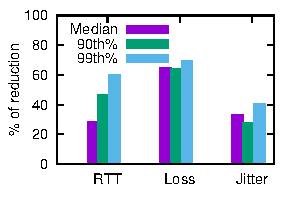
\includegraphics[width=0.45\textwidth]{figures/Via-Potential-Bar-Overall-MinChoices-5-Performance.pdf}
        \label{subfig:perf}
}
%\hspace{-0.5cm}
\subfloat[\small{Poor Network Rate}]
{
        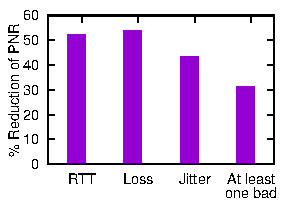
\includegraphics[width=0.45\textwidth]{figures/Via-Potential-Bar-Overall-MinChoices-5-PNR.pdf}
        \label{subfig:pnr}
}
%\hspace{-0.5cm}
%\hspace{-0.5cm}
%\subfigure[RTT]
%{
%        \includegraphics[width=0.24\textwidth]{new-figs/Potential-CDF-MinChoices-5-rRTT.pdf}
%        \label{subfig:}
%}\hspace{-0.5cm}
%\subfigure[Loss rate]
%{
%        \includegraphics[width=0.24\textwidth]{new-figs/Potential-CDF-MinChoices-5-rLOSS.pdf}
%        \label{subfig:}
%}\hspace{-0.5cm} \\
%\hspace{-0.5cm}
%\subfigure[Jitter]
%{
%        \includegraphics[width=0.24\textwidth]{new-figs/Potential-CDF-MinChoices-5-rJITTER.pdf}
%        \label{subfig:}
%}\hspace{-0.5cm}
%\subfigure[PNR]
%{
%        \includegraphics[width=0.24\textwidth]{new-figs/Potential-Bar-Overall-MinChoices-5.pdf}
%        \label{subfig:}
%}\hspace{-0.5cm}
\caption{Potential improvement of \hybrid.}
\label{fig:potential-percentile}
\end{figure}


%\begin{figure}[t!]
%\centering
%\includegraphics[width=0.4\textwidth]{new-figs/Improvement-Overall.pdf}
%\tightcaption{Improvement on mean, 90th, 99th percentiles and poor network rate (PNR) of RTT, loss and jitter. The relay path is selected for each AS pair to optimize individual metrics. 
%We also shows the fraction of reduction on fraction of calls with at least one metric being bad. }
%\label{fig:potential-percentile}
%\end{figure}

\mypara{Gains from oracle approach} Figure~\ref{fig:potential-percentile} shows the improvement (i.e., reduction) in the values of RTT, loss and jitter individually as well as the PNR (defined in Section~\ref{subsec:measurement:voip:method}). Specifically, if 
% the values in the dataset currently and after our decisions are
a statistic goes from  $b$ to $a$, we define the {{\em relative}} improvement as $100 \times (\frac{b-a}{b})$, which lies between $0$ and $100$. %\vnp{I presume Fig 9(a) shows the percentage reduction in the actual metrics, and Fig 9(b) the reduction in the PNR. If this is incorrect, the text here as also at the beginning of Sec 3 needs to be edited accordingly.}
%For each AS pair, we select the relay path to optimize individual metrics. The distribution of resulting performance is obtained by combining real performance measurements of the path picked for each AS pair and weighted by the population of each AS pair. 

The oracle can help reduce RTT, loss and jitter by $30\%$-$60\%$ at median (Figure~\ref{subfig:perf}). Reduction at the tail, which is of particular significance in interactive services,
% importance in production, 
is nearly  $40\%$-$65\%$ with the oracle's choice of relaying. All this translates to a healthy reduction in the PNR on each of RTT, loss, and jitter (Figure~\ref{subfig:pnr}, left three bars) of up to $53\%$. Source-destination pairs with fewer calls between them have a lower impact on the PNR and its improvement. 

We also analyze the reduction in PNR when the three metrics are considered {\em together}, i.e., improving from a situation where at least one of the metrics is poor to a situation where {\em none} of the three is poor (i.e., RTT $\leq 320$ms, loss $\leq 1.2\%$, {\em and} jitter $\leq 12$ms), while still optimizing for RTT, loss and jitter individually. %This helps us understand how correlated is the improvement in the three metrics. 
Even while optimizing for each of the three metrics, we can obtain a PNR for ``at least one bad'' metric; we conservatively pick the {\em worst} among the three for our analysis. Despite this strict stipulation, we can achieve reduction of over $30\%$ in PNR (Figure~\ref{subfig:pnr}, right-most bar).

\begin{figure}[t!]
\centering
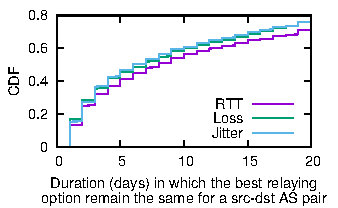
\includegraphics[width=0.5\textwidth]{figures/Via-Potential-PersistenceOfOracleDecision.pdf}
\caption{Distribution of how long the best \option (picked by oracle) lasts. The optimal \options for $30\%$ of AS pairs last for less than $2$ days.}
\label{fig:potential-persistence}
\end{figure}

\mypara{Need for dynamic relay selection} 
Whether the controller should select relay dynamically depends on how often the relaying decisions need to be updated. 
Figure~\ref{fig:potential-persistence} shows the distribution of the median duration during which the oracle picks the same \option for a source-destination AS pair.
%For each source-destination AS pair, persistence is defined by the median consecutive days during which oracle picks the same relay option. 
The optimal \option for $30\%$ of AS pairs lasts for less than $2$ days, and only $20\%$ of AS pairs have the same optimal relay option for more than $20$ days. 
This, together with the observation on the relatively low persistence of poor performance (Figure~\ref{fig:temporal-structure}), suggests that the relay selection should be done {\em dynamically}, rather than statically.

